\section{Methods}
\label{Methods}
% This should be fairly brief, the system is not particularly complex.
For the SORA flights, the MiniPIX was interfaced via USB with a Raspberry PI single board computer (RPI). Data was collected on the MiniPIX and frame data was sent over serial to the RPI for analysis. During the 2017 flight, only the raw data was stored for post-flight analysis. For the 2018 flight, a custom piece of software was written to concurrently handle analyzing frame data, calculating absorbed dose and handling command and configuration requests from the HASP telemetry interface in addition to storing the raw data. The improvements in the 2018 flight allowed for a near real-time analysis of the radiation environment and the ability to configure the MiniPIX shutter rate and detector parameters via the HASP uplink interface. While being relatively cheap at a price point of 35\$ USD and consuming only \SI{X}{\watt} the RPI proved to be robust and operated without glitch for the duration of both flights.



\subsection{Configuration and Calibration}
% Device parameters, threshold, bias voltage, shutter time etc.
The Timepix ASIC consists of 65,536 silicon p-n diodes, with each containing its own individual processing circuit. The response of each pixel can never be identical, thus a calibration must be performed for each individual pixel. The appropriate calibration of the MiniPIX detector was applied at The University of Houston following a calibration procedure outlined by Jakubek \cite{mpjakubek}. The source calibration was applied using the 60 keV $^{241}$Am decay line, Sn Fluorescence and $^{55}$Fe gamma rays.

\subsection{System Design}
% RPI interface to MiniPIX, heatsink design etc.
Additive manufacturing was utilized to create a custom made case for the MiniPIX device.  As seen in Figure ~\ref{fig:minipix_case}, the MiniPIX case is in white, while the heat sink setup is in blue-gray color.  In the early vacuum tests, it was found that the MiniPIX would require a passive cooling method to keep the device at operational levels.  At the same time, the ABS plastic enclosure acted as insulation, maintaining the MiniPIX temperatures in operational ranges.  The MiniPIX device was mated to the heatsink via a bracket (not shown in the figure ~\ref{fig:minipix_case}) and with thermal adhesive.
\begin{figure}[H]
    \centering
    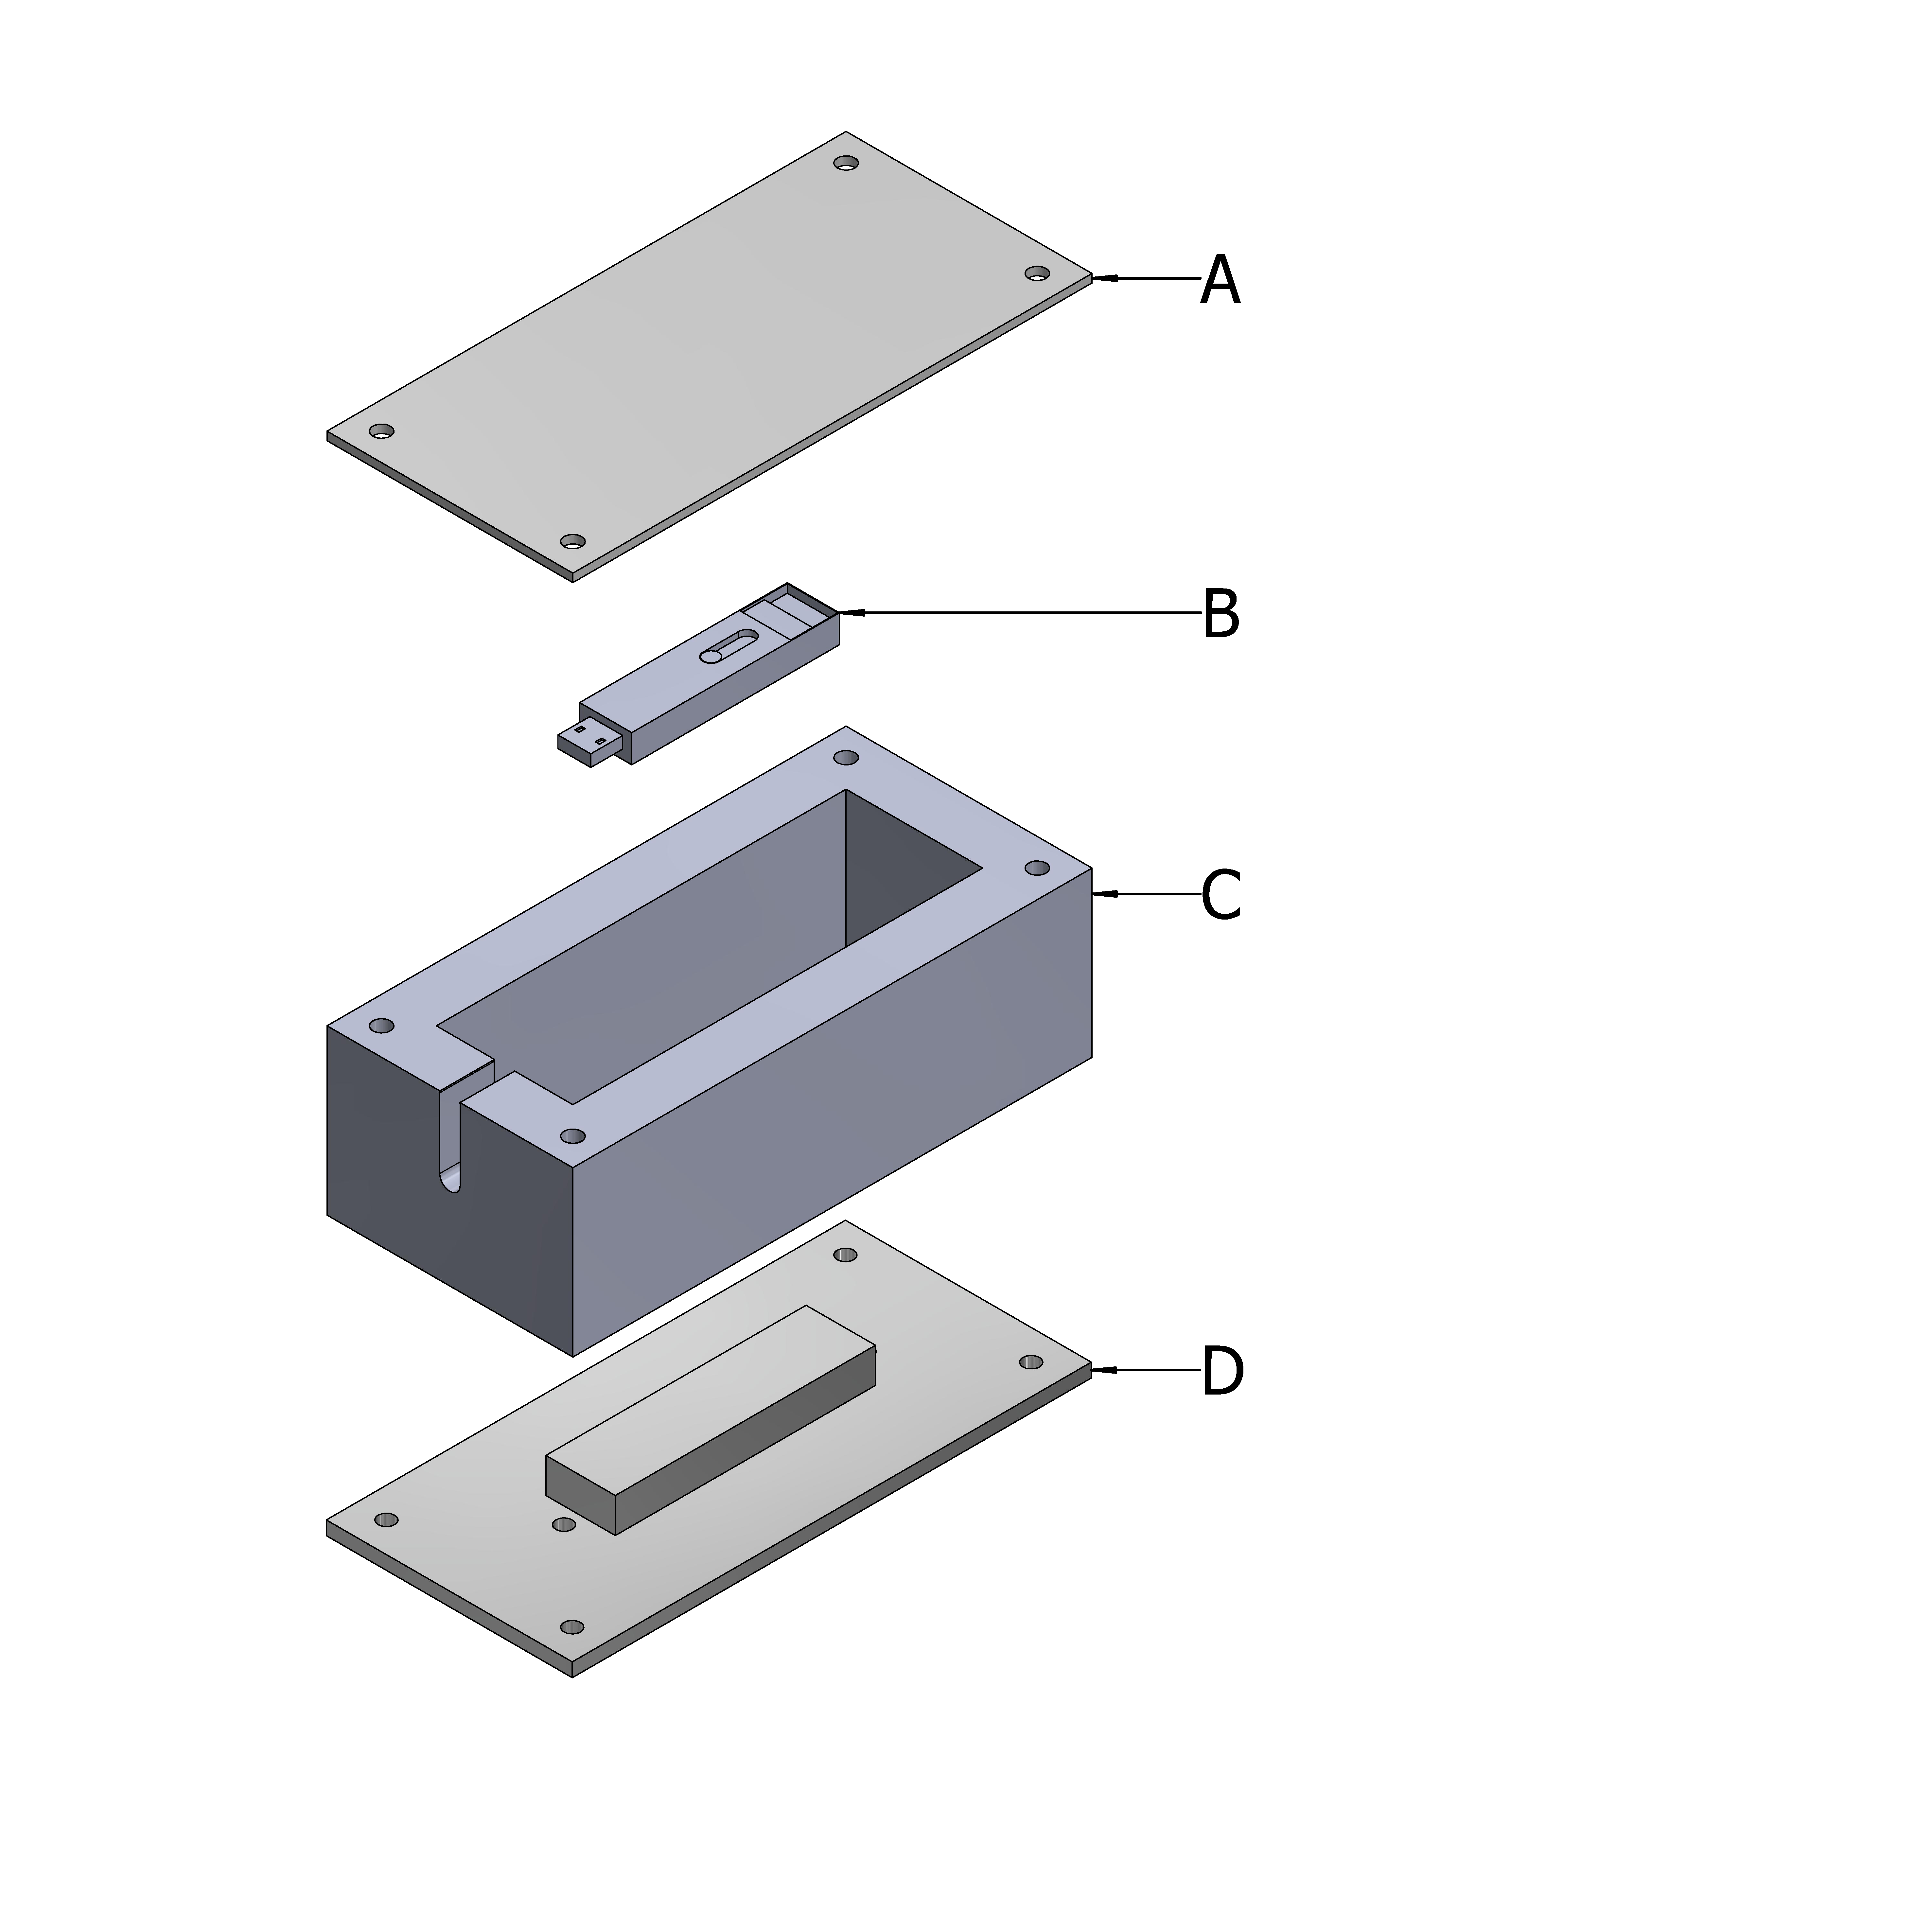
\includegraphics[width=0.50\textwidth]{Minipix_case_assembly.pdf}
    \caption{MiniPIX Case Assembly}
    \label{fig:minipix_case}
\end{figure}
The MiniPIX case allowed for a USB cable to be routed through the enclosure to interface directly to the Raspberry Pi.  This allowed the MiniPIX device to be modular and be place in different configurations for both flights.  The Raspberry Pi was placed in a separate location within the payloads near the power supply.  Overall, the payload was modular and accessible.



